\section{\heiti 相关工作}
在数据和算力受限的背景下,LJP的早期探索主要依赖统计学方法。
例如,Kort~\cite{kort1957predicting} 通过多因素复合分析,揭示了美国最高法院处理特定案件时的判决规律。
该时期的研究还包括应用专家系统将法律知识转化为计算机可处理的规则~\cite{susskind1986expert}。
然而,这些传统方法的核心局限在于它们对噪声数据的高度敏感性以及对人工规则的过度依赖。
法律文本的复杂性和模糊性使得规则制定和特征标注异常困难。
简单的数学模型难以捕捉司法实践中复杂多样的非线性影响因素,从而限制了其预测性能和泛化能力~\cite{deng2023syllogistic,dong2021legal}。


为解决此问题,研究转向了机器学习和文本挖掘技术~\cite{chen2013text,goncalves2005evaluating}。
学者们通过将案件事实作为输入、判决结果作为标签,利用支持向量机(SVM)~\cite{kianmehr2006crime} 或随机森林(Random Forest)~\cite{sulea2017exploring}等模型,从案情描述中自动学习特征以预测判决。
例如,Katz等~\cite{sulea2017exploring} 应用随机森林模型,有效提取了影响美国最高法院判决的关键特征。
这类方法的优势在于增强了模型对非线性关系的建模能力,并初步实现了特征提取的自动化。
然而,其短板也十分明显:模型性能高度依赖于人工设计的特征工程,这不仅耗费大量人力,而且难以挖掘文本背后深层次的语义信息,导致其难以迁移至更广泛的法律场景。


随着深度学习的兴起,LJP研究迎来了新的突破。
基于深度神经网络的模型能够自动捕捉文本中更复杂、更抽象的特征~\cite{cheng2025legal,feng2022legal,jiang2018interpretable,wang2019hierarchical}。
Luo等~\cite{huang2019improved} 提出的模型利用注意力机制,动态识别并聚焦于事实描述中最关键的部分,有效关联了案件事实与罪名认定,显著提升了预测准确性。
为了更全面地模拟司法过程,Yue等~\cite{yue2021neurjudge} 构建了一个情境感知的多任务学习框架(NeurJudge),它通过协同法条预测、罪名预测等多个子任务,使模型学习到任务间的共享信息,从而提升了主任务的性能。
受BERT等模型成功的启发,法律AI领域涌现出Legal-BERT~\cite{liu2021robustly,chalkidis2020legal,deepa2021bidirectional,devlin2019bert,fan2022multi}、Lawformer~\cite{xiao2021lawformer,du2022glm,fei2023lawbench,oana-maria2018e-snli}等在海量法律语料上预训练的模型。
它们通过迁移学习,将从大规模无标注文本中学到的丰富语言知识应用于下游任务,相较于传统机器学习模型,获得了显著的性能提升~\cite{cui2021pre,houlsby2019parameter,hu2018few,zhang2023contrastive}。
尽管深度学习极大地推动了LJP的发展,但深度学习模型如同“黑箱”般运作,其决策过程缺乏透明度和可解释性。尤其当数据存在潜在偏见时,深度学习模型可能直接导致不公正或不一致的判决结果。


\begin{figure*}[htpb]
	\centering
	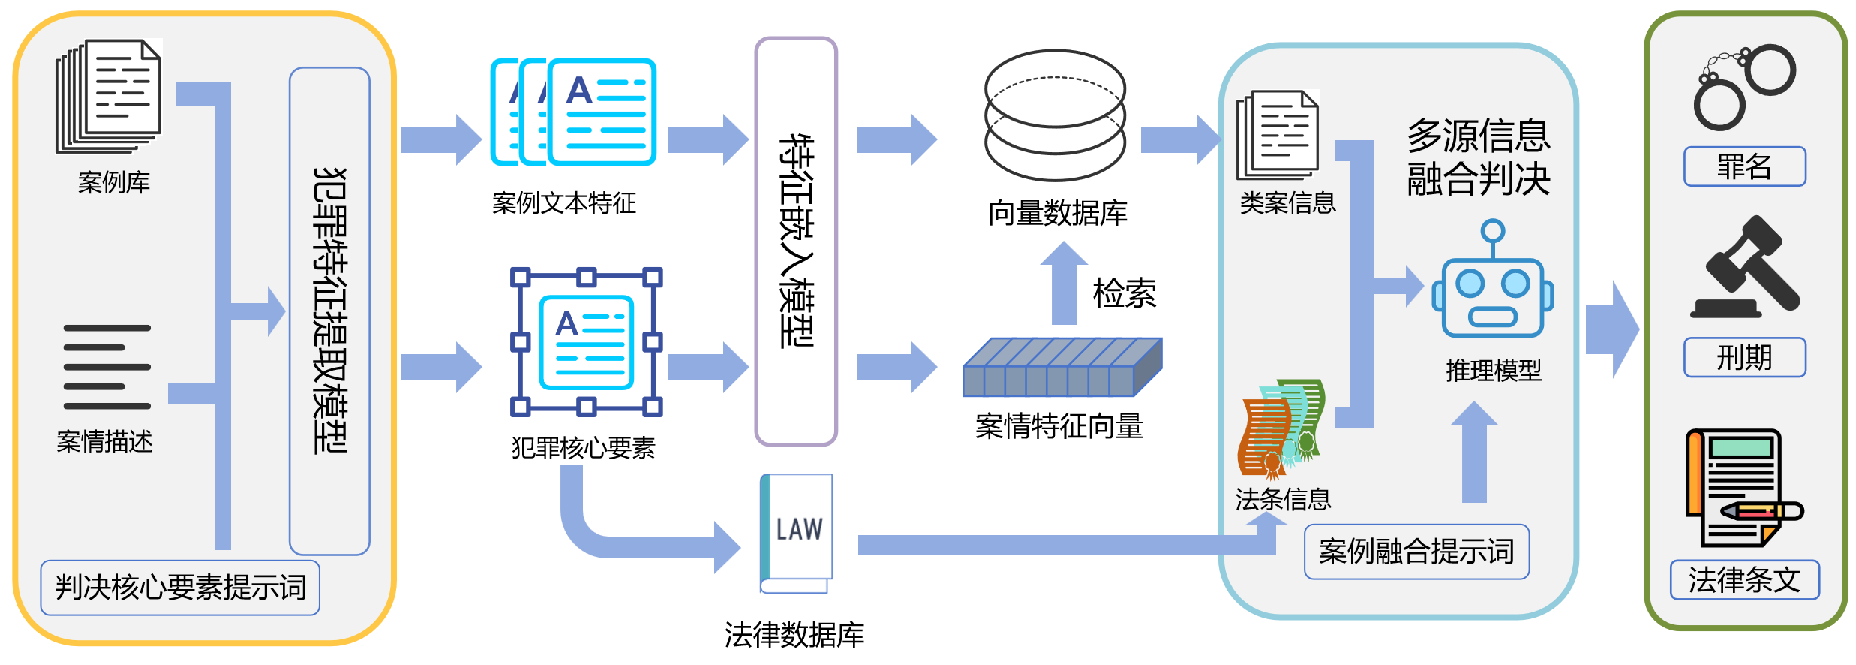
\includegraphics[width=1\textwidth]{fig/method2.pdf}
	\caption{基于法条约束与类案融合的可解释司法判决预测方法}
	\label{fig:main}
\end{figure*}

LLM因其强大的复杂上下文推理能力、庞大的预训练知识库和良好的可解释性,被期望成为下一代LJP的新范式~\cite{wu2020de-biased,yang2023baichuan,yao2020refining}。
当前,以LLM为核心的技术范式已成为研究热点。其强大的常识推理和零样本/少样本学习能力为LJP带来了新的可能性~\cite{brown2020language,huang2022towards,shu2024large,wen2024review}。
将LLM直接应用于严肃的法律领域仍面临严峻挑战。
未经充分优化的通用LLM在处理法律问题时,容易出现“幻觉”(Hallucination)~\cite{cui2023survey,radford2025improving,raffel2020exploring}。这可能表现为捏造不存在的法律条文、引用错误的案例,或给出超出法定范围的量刑建议~\cite{lewis2020retrieval}。
为解决LLM的幻觉问题,主要优化思路分为两条路径。一是通过提示工程(Prompt Engineering)引导模型,例如利用“思维链”(Chain of Thought)~\cite{kojima2022large,izacard2021leveraging,rajani2019explain,talmor2019leap,wang2023self,wei2022chain}或司法三段论~\cite{huang2023lawyer,trautmann2022legal,xu2023superclue,yu2022legal}来规范其推理逻辑。
然而,为特定任务精心设计的提示词(Prompt)往往缺乏通用性,难以直接迁移至其他法律任务,这限制了其可扩展性;
二是以法律专业数据对LLM进行微调,例如Lawyer LLaMA~\cite{chen2020recall,yue2021circumstances},使其具备更强的“法律素养”。
尽管微调是提升专业性的有效途径~\cite{hu2021lora,hu2022lora,zelikman2024star},但LLM微调存在以下问题:首先,微调的成功依赖于高质量标注数据和大量计算资源。
其次,微调后的LLM知识体系是静态的,其知识停留在训练数据集的时间点,无法实时跟进法律法规的更新和司法解释的演进~\cite{li2021prefix,zhang2024comprehensive}。
最后,微调过程还可能导致模型对其通用知识的“灾难性遗忘”~\cite{chen2020recall},损害其基础推理能力。
因此,本研究提出一种基于LLM并由法律引导的案例融合方法。
该方法将提示词工程与检索增强技术相结合,以实现司法智能审判的可信判决。
该方法通过特定的提示词提取案例描述的关键判决核心要素,从而保留司法审判理论的核心要素并去除冗余噪声。
此外,通过引入案例数据库和法律条文数据库,为LLM提供精确的罪名定义和司法实践案例,以综合理论知识与实践经验。
最后,利用多源异构信息进行综合分析与推理,做出最终的司法判决。
该方法无需微调LLM,并且可以通过引入新的法律条文和案例,提供最新的法理知识,从而避免LLM因缺少相关知识而产生幻觉。


